\section{Our \ApproachName{} Approach} 
\label{sec:Approach}

This section will explain how our approach makes use of evolutionary computation to transplant elements within video games content. We first present an overview of our approach and subsequently provide the details of
the approach. To help the reader, we provide along with the approach explanation a theoretical example of auto-transplantation of content within a simplified version of \sq{bosses} of the video game \CaseStudy{}.

Figure~\ref{fig:approach} shows an over of our approach.
Our approach is named after Imhotep, who is considered by many to have written the Edwin Smith papyrus (the oldest known manual of surgery)\footnote{\url{https://www.pastmedicalhistory.co.uk/imhotep-the-first-physician/}}.
On top of the figure we show the input to our approach, which is the organ to be transplanted from the donor and the hosts where the organ will be transplanted. Afterwards, Imhotep detects the points of the organ that allows the transplantation and the points where the organ can be inserted. To initialize the population of the evolutionary algorithm, the organ is transplanted in a random point and cloned. When the evolutionary algorithm finish the execution we obtain a ranked list by the objective function of the best transplantation between organ and host.

\begin{figure}[h]
    \centering
    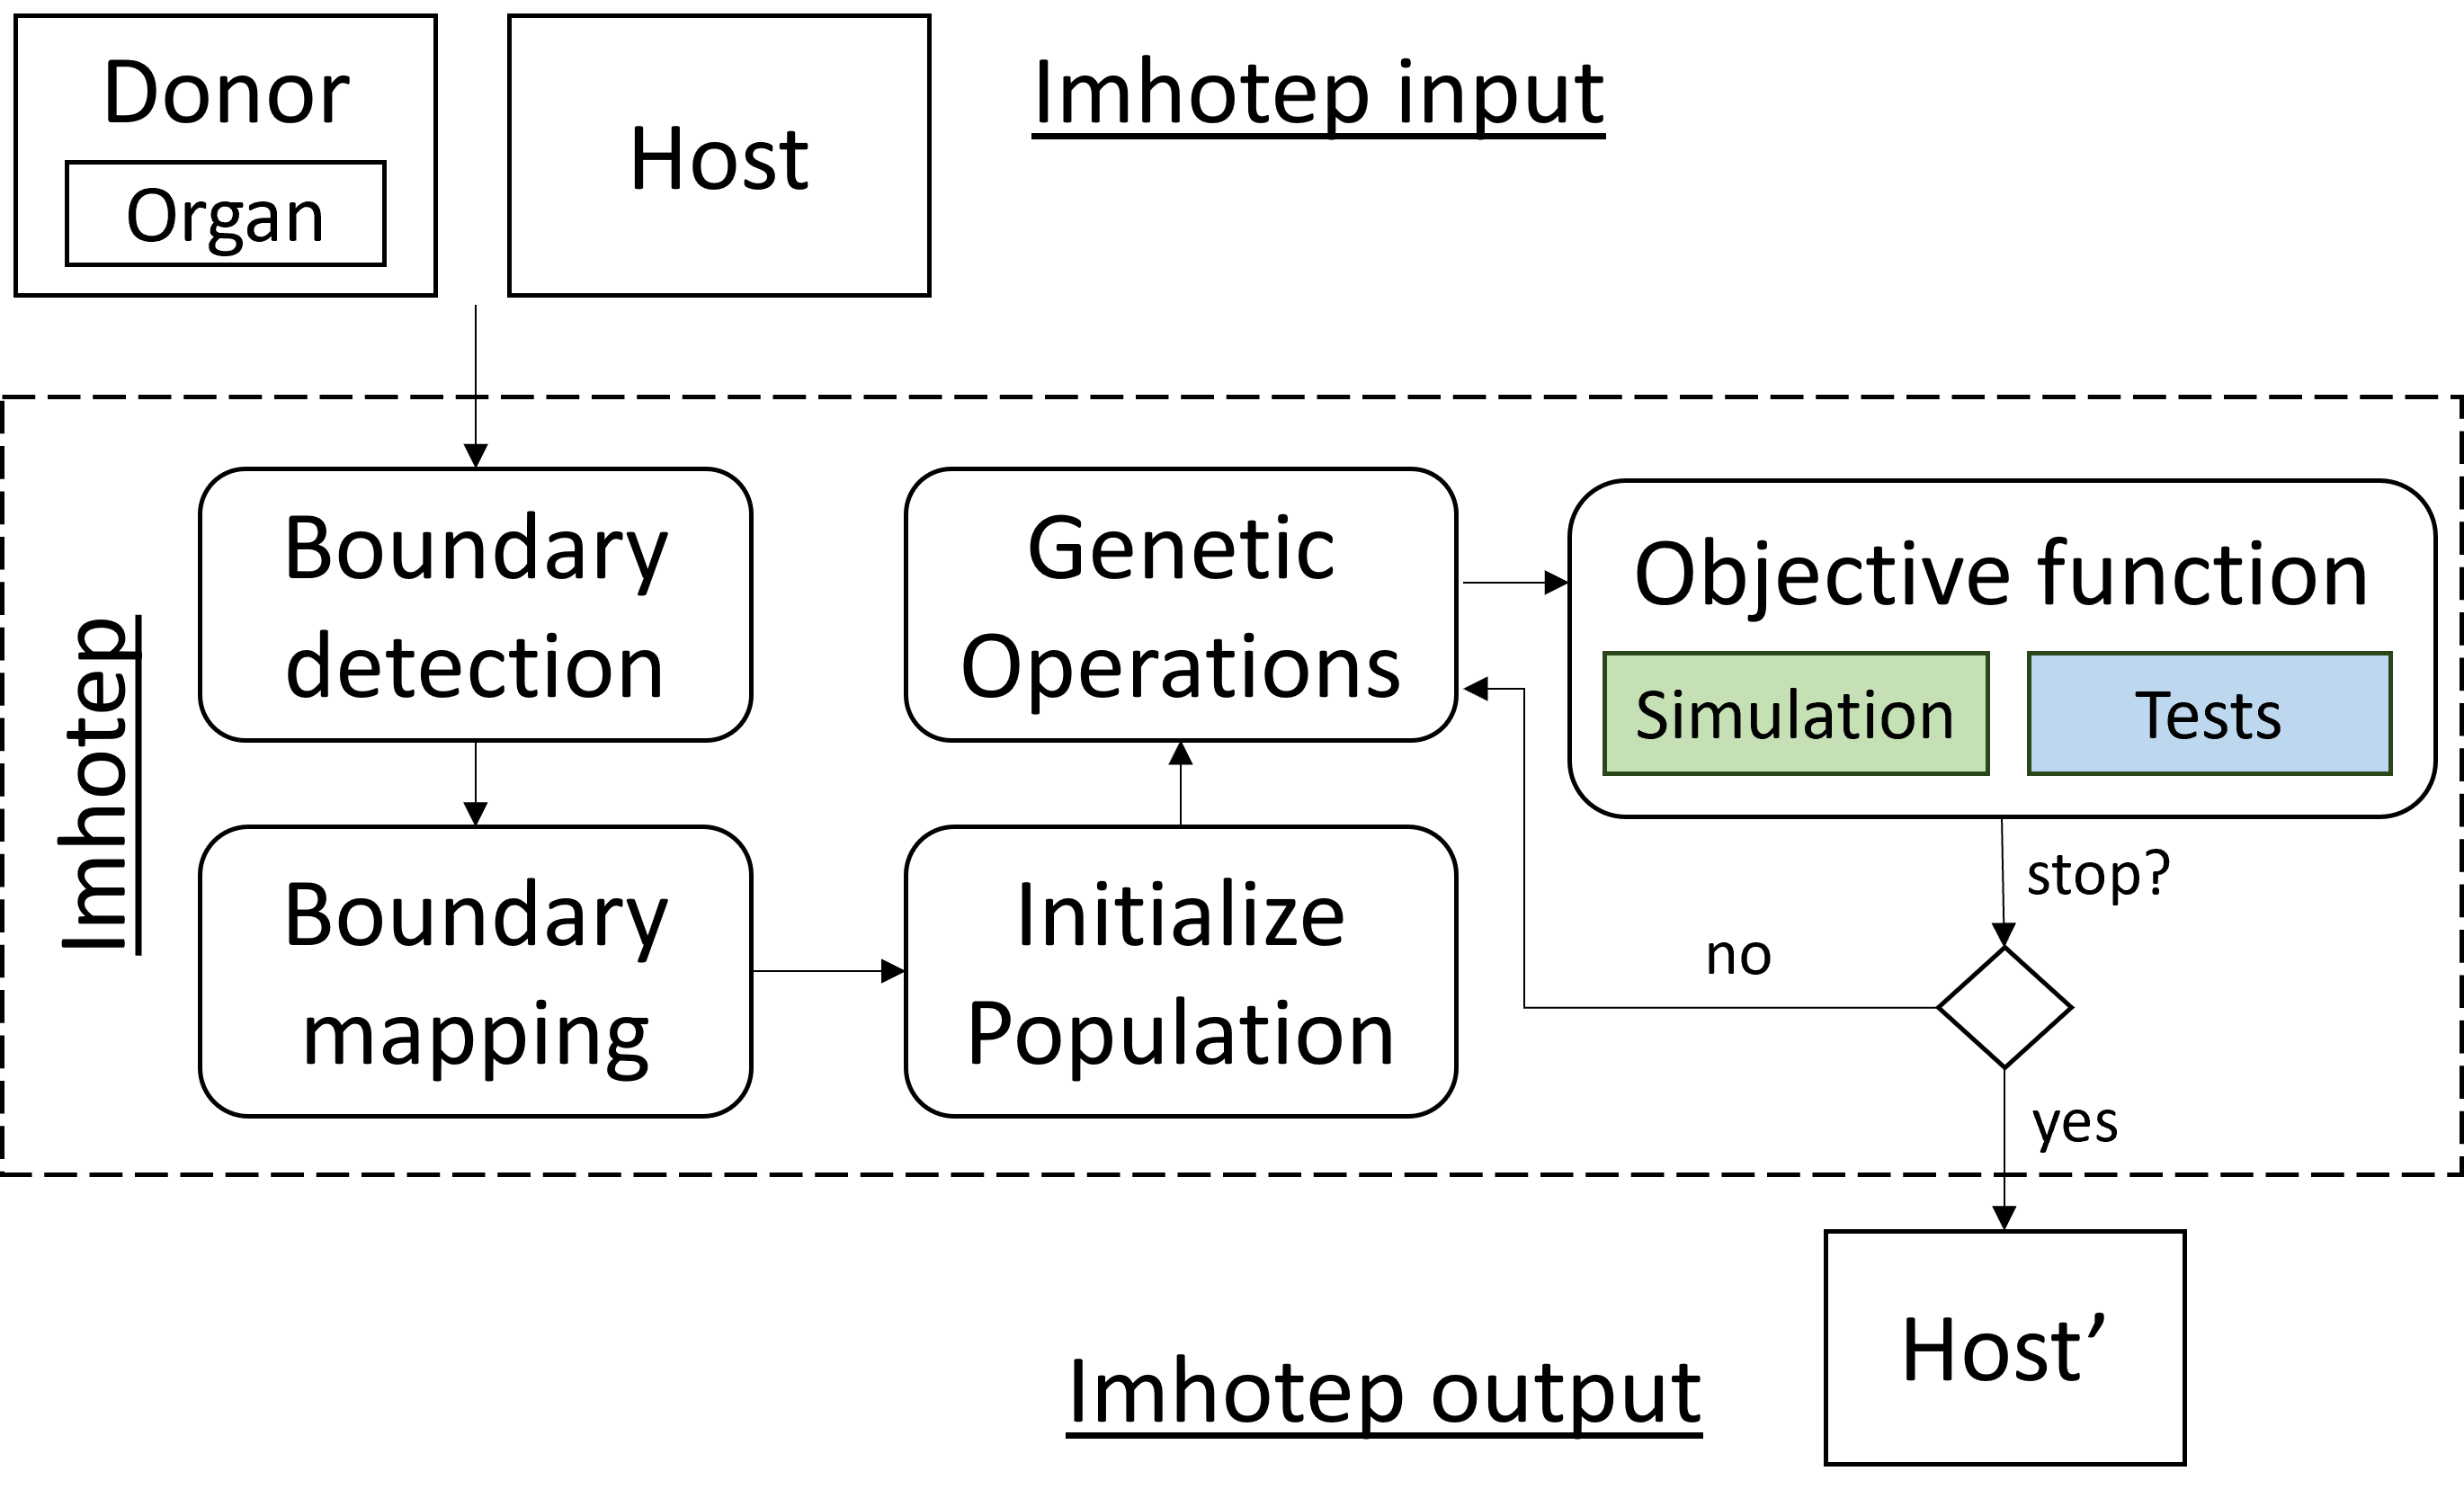
\includegraphics[width=0.45\textwidth]{Figures/overview.png}
    \caption{Overview of Imhotep}
    \label{fig:approach}
\end{figure}


\subsection{Input selection}

The very first step of our approach is the definition of the input. \ApproachName{} requires the developers to define a source model content (donor) with the organ that will be transplanted, and a target model content (host). The models used in \ApproachName{} are models based on SDML as explained in the background section (\ref{sec:Background}). The donor and host from the example are different from the donor and host used in the evaluation, but we think they will help to understand the approach. The donor, organs and host used by \ApproachName{}

In our example we present a simplified version of the metamodel, and the corresponding concrete syntax of the model (Fig.~\ref{fig:metamodel+syntax}) from the video game \CaseStudy{}. In this example we use a graphical representation to help the comprehension of the reader. Notice that the original metamodel does not work with a graphical model representation as it is not a requirement on every metamodel. The type of model will depend on the metamodel and models that developers decide on.

\begin{figure}[h]
    \centering
    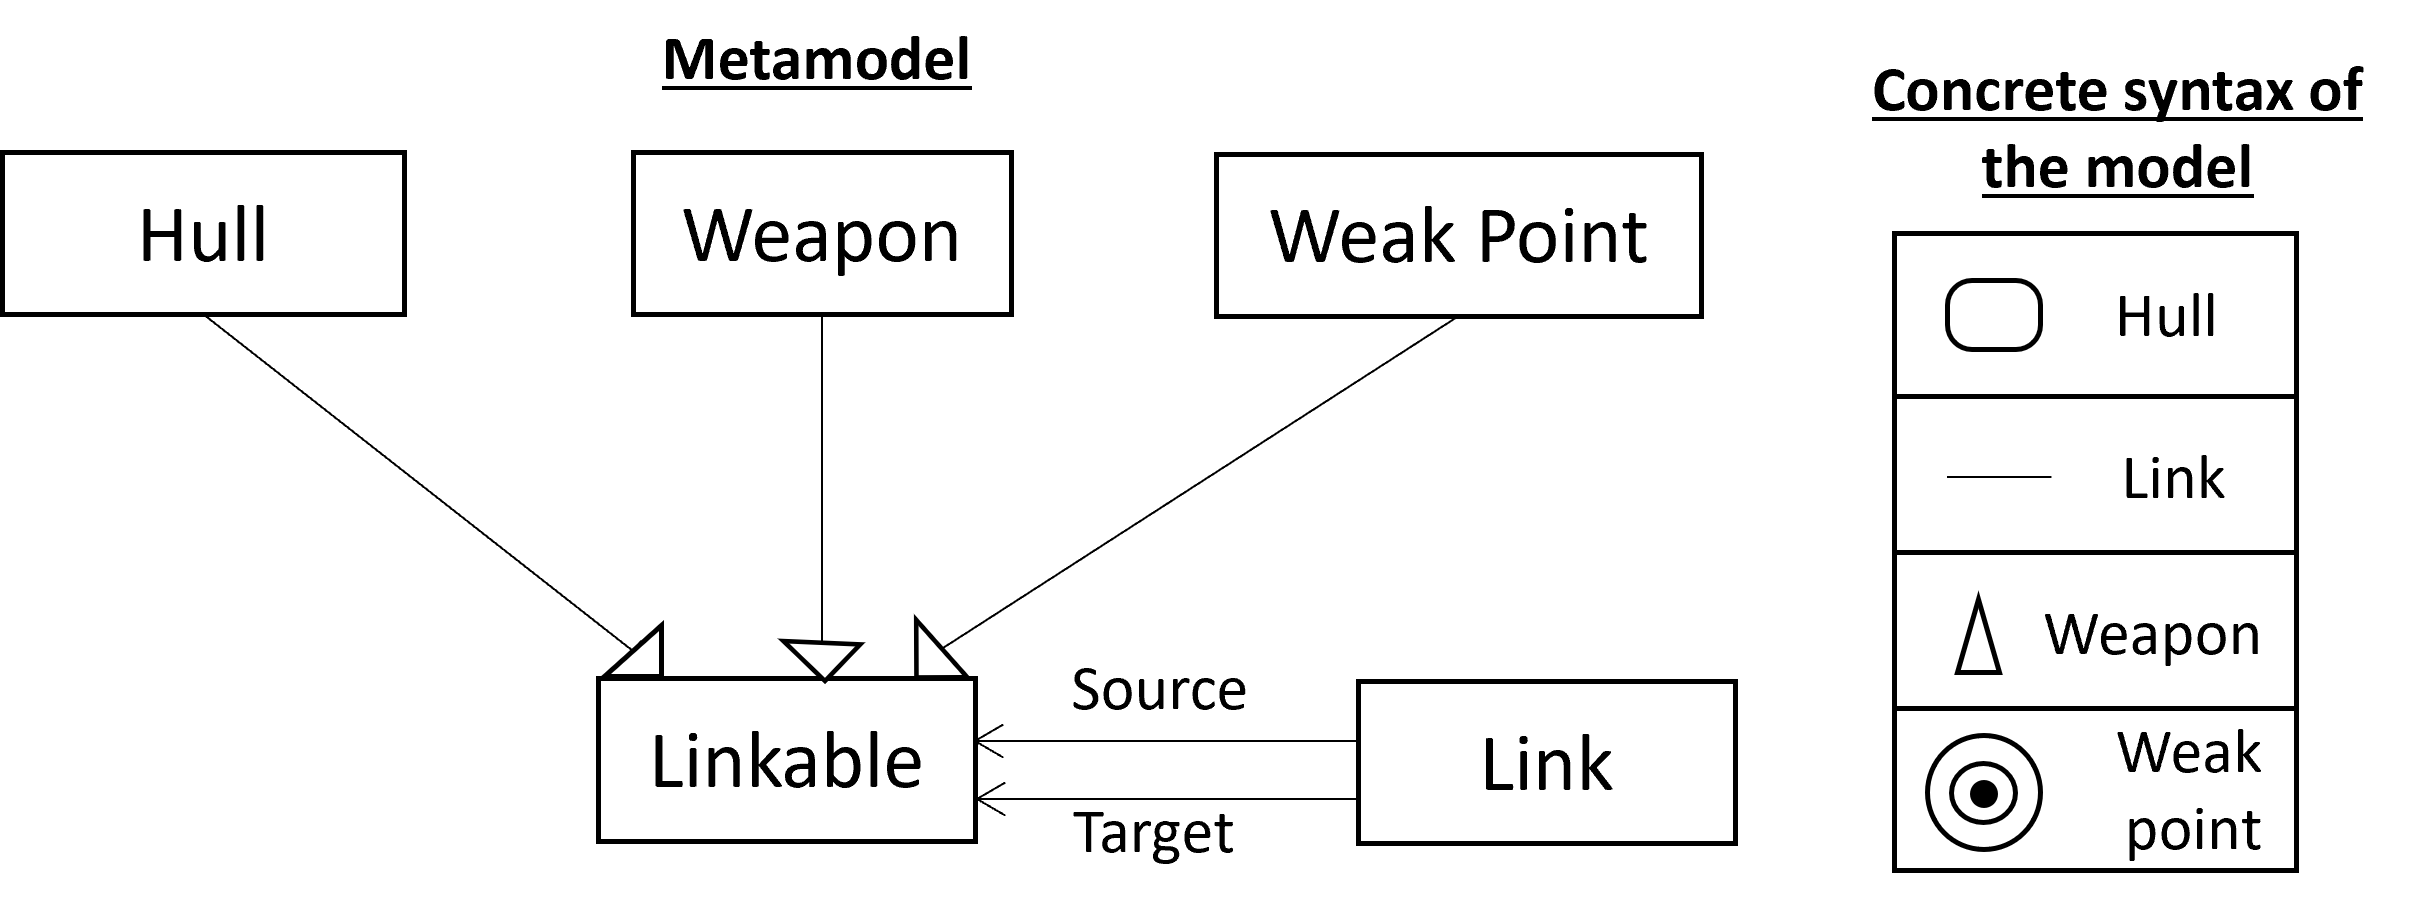
\includegraphics[width=0.45\textwidth]{Figures/metamodel+syntax.png}
    \caption{Simplified metamodel with the corresponding concrete syntax of the model.}
    \label{fig:metamodel+syntax}
\end{figure}

Based on the metamodel of our example, we define the inputs as stated. 
First, we define the source donor, that is a simplified version of an original \sq{boss} from \CaseStudy{}, called \sq{Serpent} (Fig.~\ref{fig:donor}). The original model is a SDML model written on a XML file with approximately 1700 lines of code. Figure~\ref{fig:donor} shows the graphical representation of the donor, differentiating each element of the model with a letter from A to S. It also shows in green the elements selected as organ (the elements H, I, J, K, N, O, P, Q).
Secondly, we define the host of our example. To that extent, we have created a regular enemy that could appear in \CaseStudy{} following the metamodel (Fig.~\ref{fig:host}.

\begin{figure}[h]
    \centering
    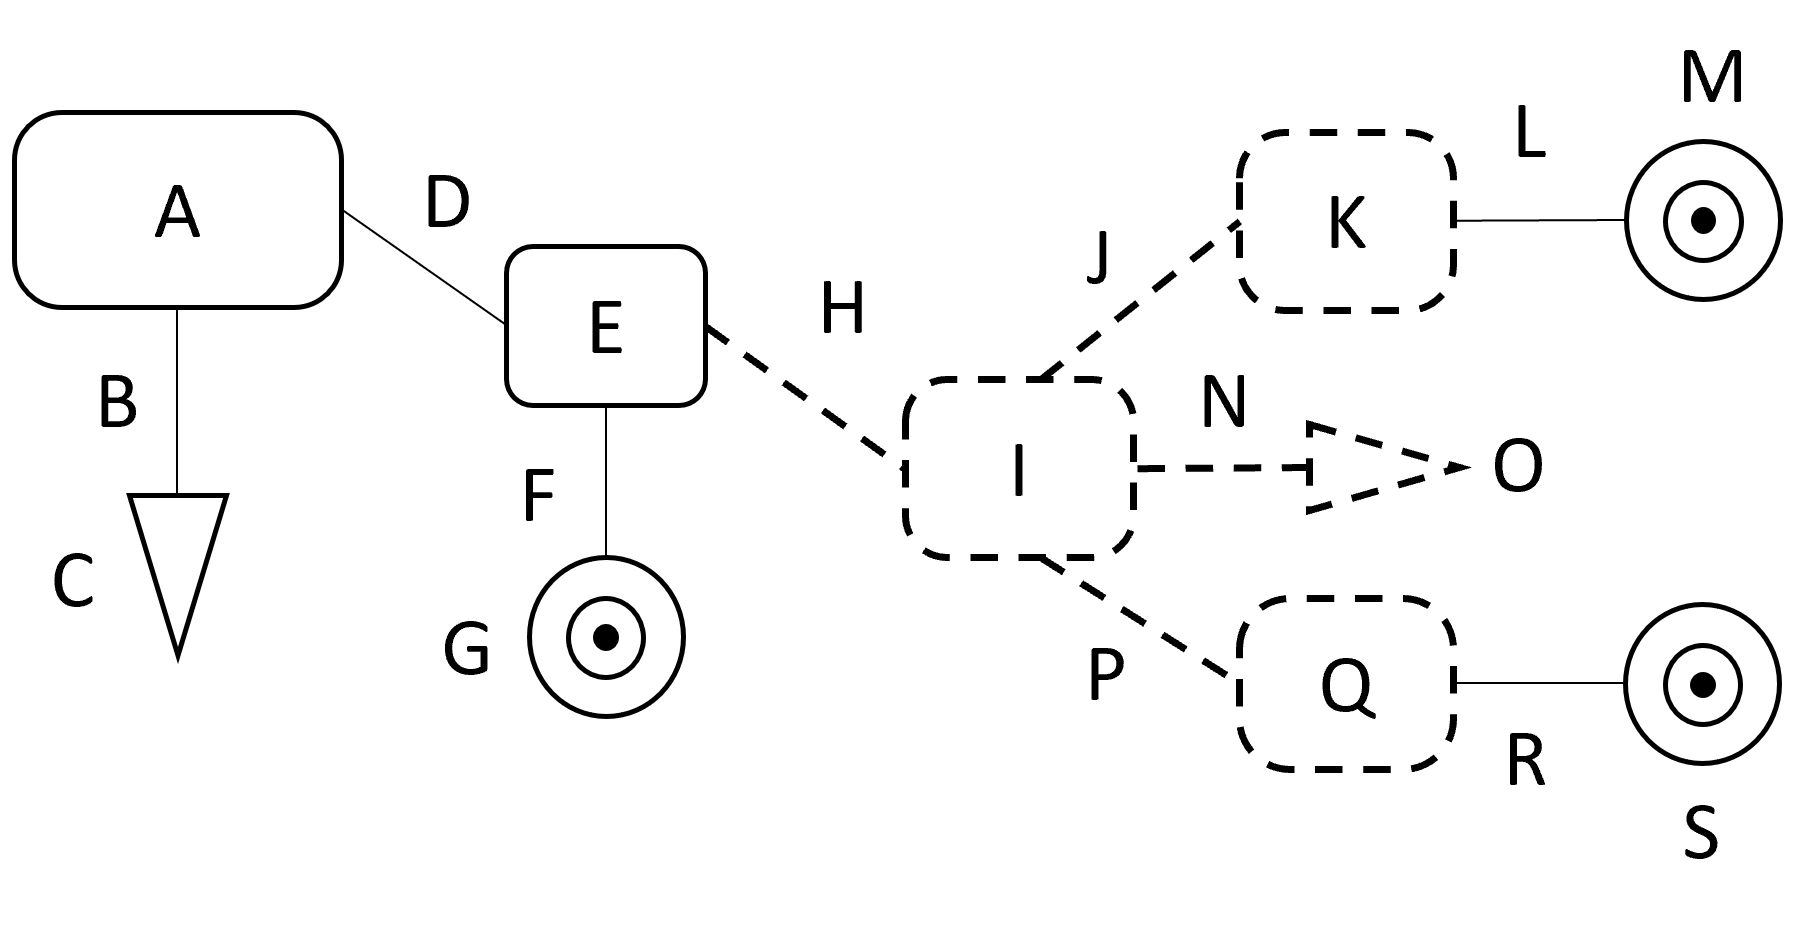
\includegraphics[width=0.45\textwidth]{Figures/donor+organ.png}
    \caption{Donor with organ selection in doted lines. The letters represent each element of the model.}
    \label{fig:donor}
\end{figure}

\begin{figure}[h]
    \centering
    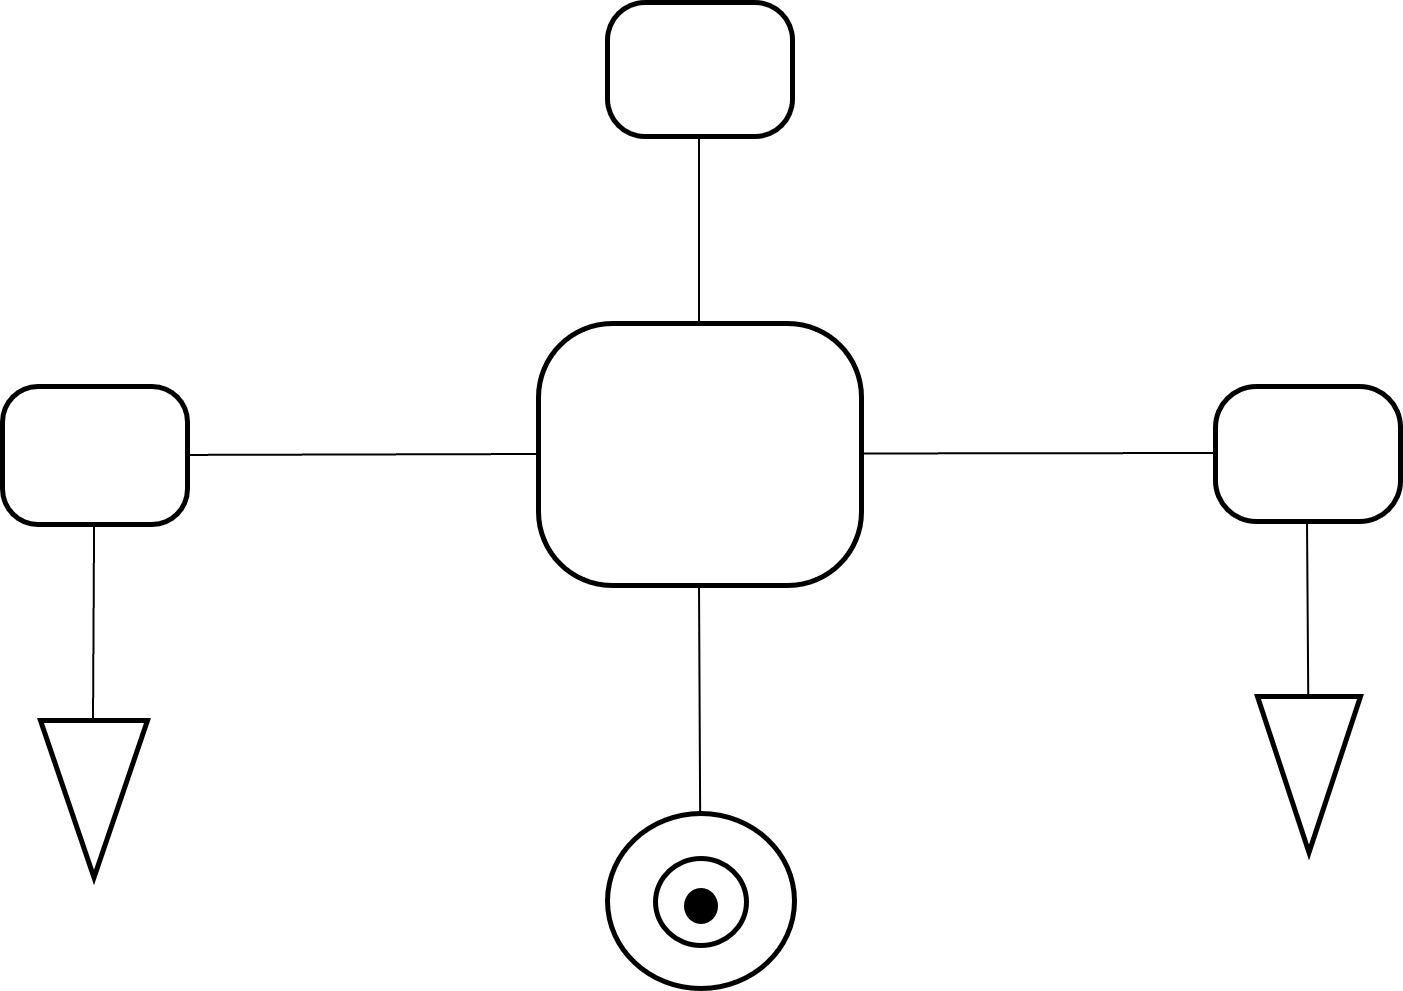
\includegraphics[width=0.3\textwidth]{Figures/host.png}
    \caption{Host}
    \label{fig:host}
\end{figure}

\subsection{Boundary detection}

To transplant an organ into a host we need to find a way to connect them. To do that we use the boundaries of the organ and the host. A boundary is a connection point on an element capable of connecting two distinct elements within a model. The connection is restricted by the rules of the metamodel. \ApproachName{} automatically identifies the boundaries of the selected organ, and all the boundaries of the host before initializing the evolutionary algorithm.

Following our example the approach will detect the boundaries of the organ, and the host. The boundaries of the organ will be the connection points between donor and host. The elements that connect with the rest of the donor are H, K, and Q. We can then state the boundaries on each element. Figure~\ref{fig:org_bound} shows the donor, the organ, and the boundaries (boundaries are represented by a circle crossed). The boundaries of the organ will be; b11 for the H element; b16 for the K element, and b25 for the Q element.

\begin{figure}[h]
    \centering
    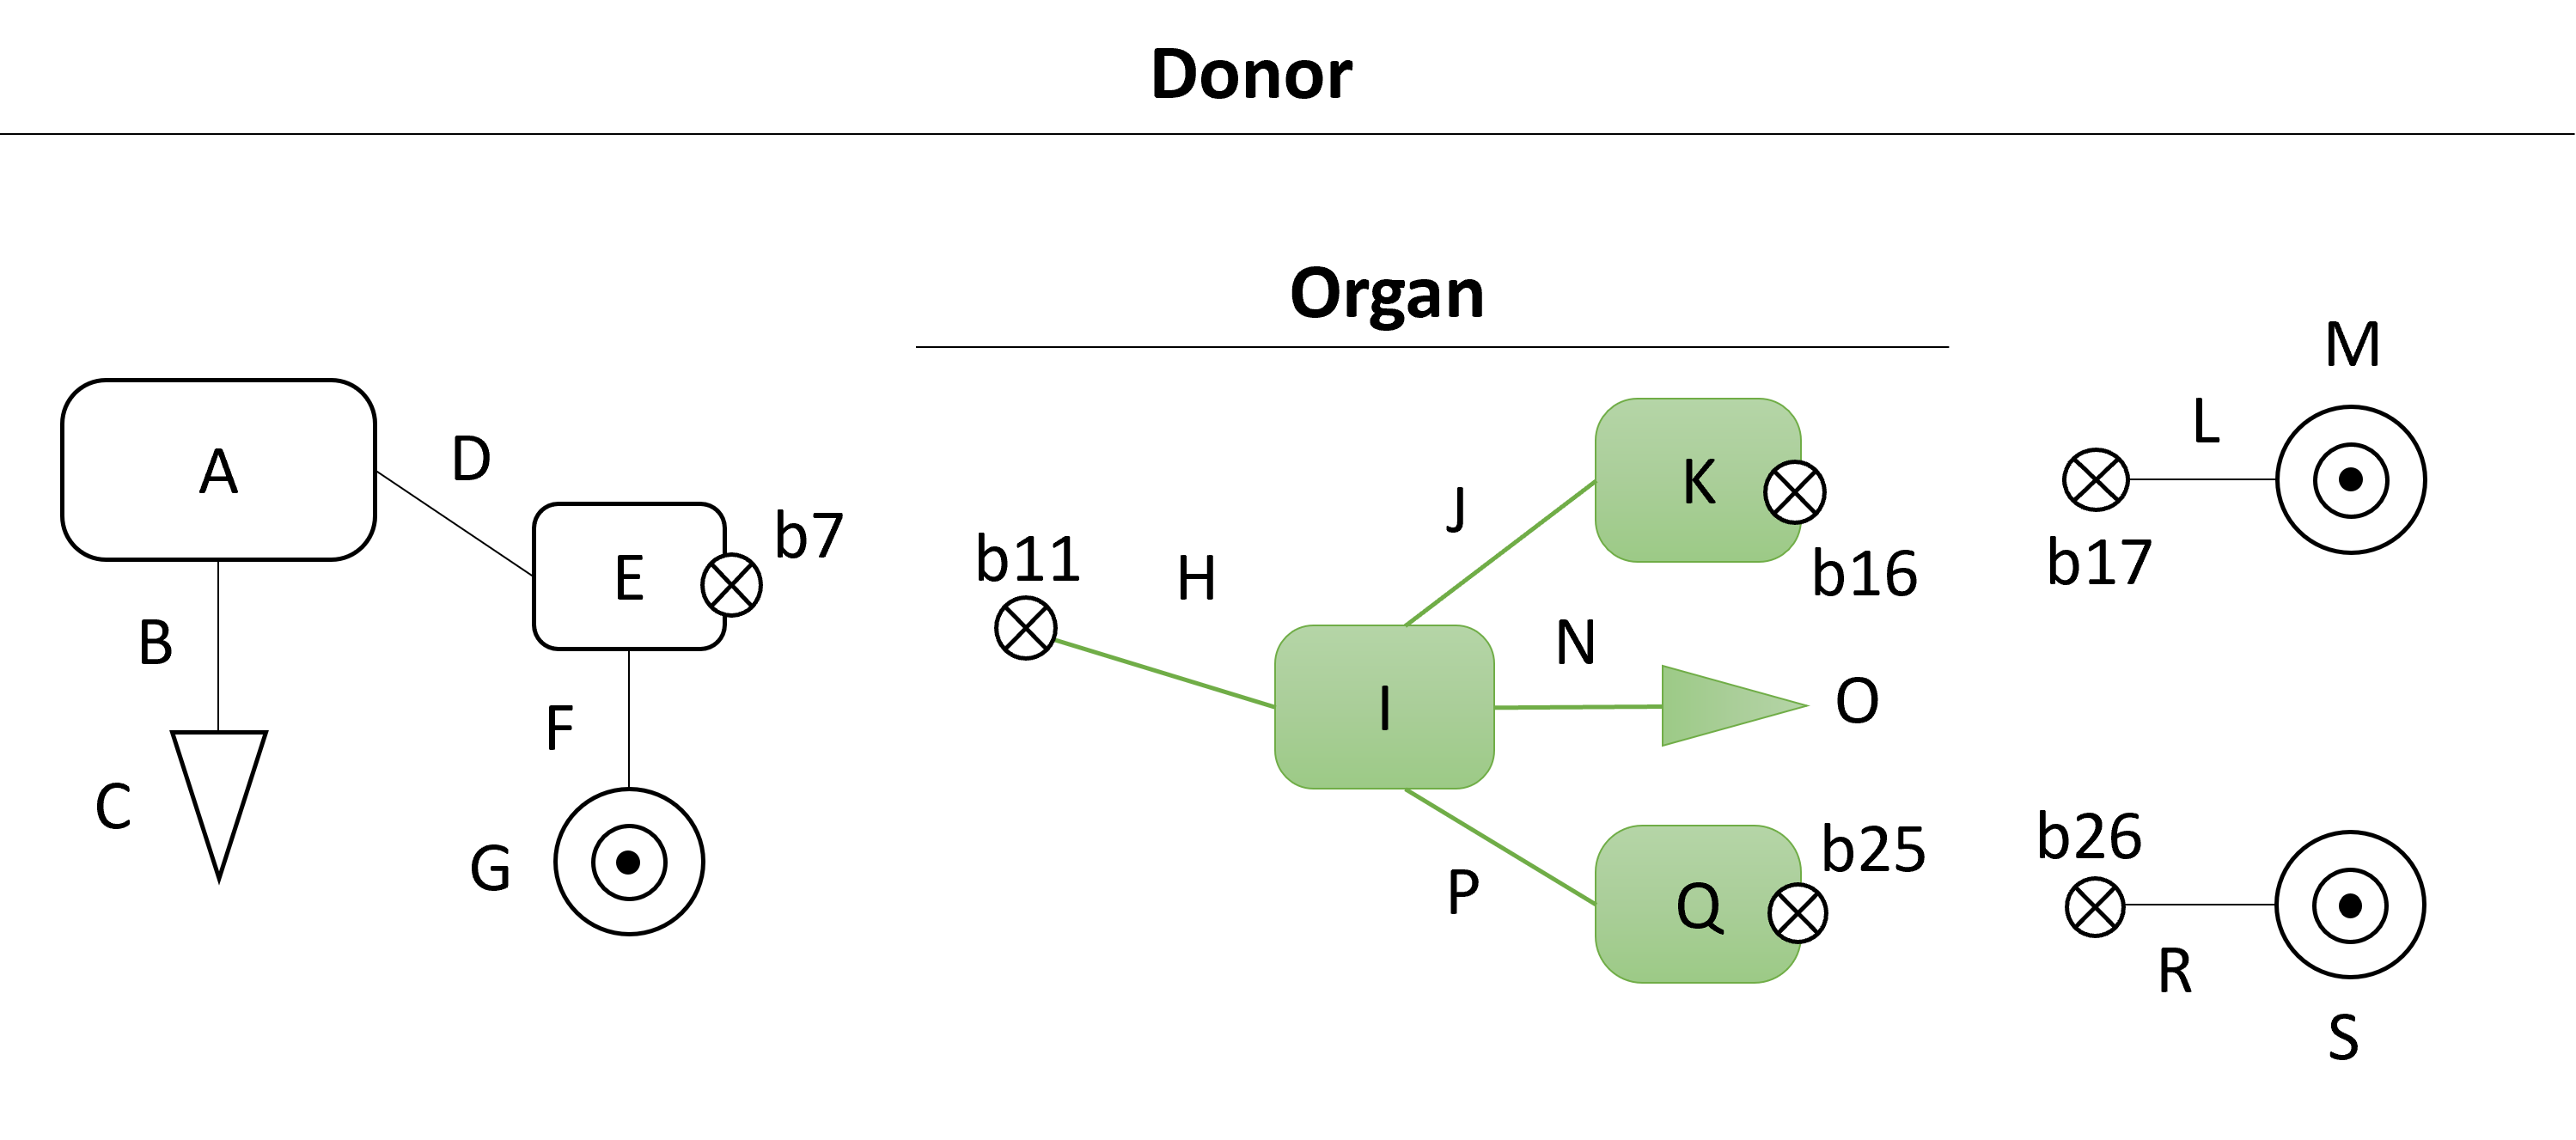
\includegraphics[width=0.45\textwidth]{Figures/donor+organ_boundaries.png}
    \caption{Definition of organ boundaries. The boundary is represented by a circle crossed.}
    \label{fig:org_bound}
\end{figure}

On the other hand, the boundaries of the host will be all the points where its elements connect. Figure~\ref{fig:host_bound} shows all the boundaries of the host of the example. The host has a total of 19 boundaries identified by a tag from ba to bs.

\begin{figure}[h]
    \centering
    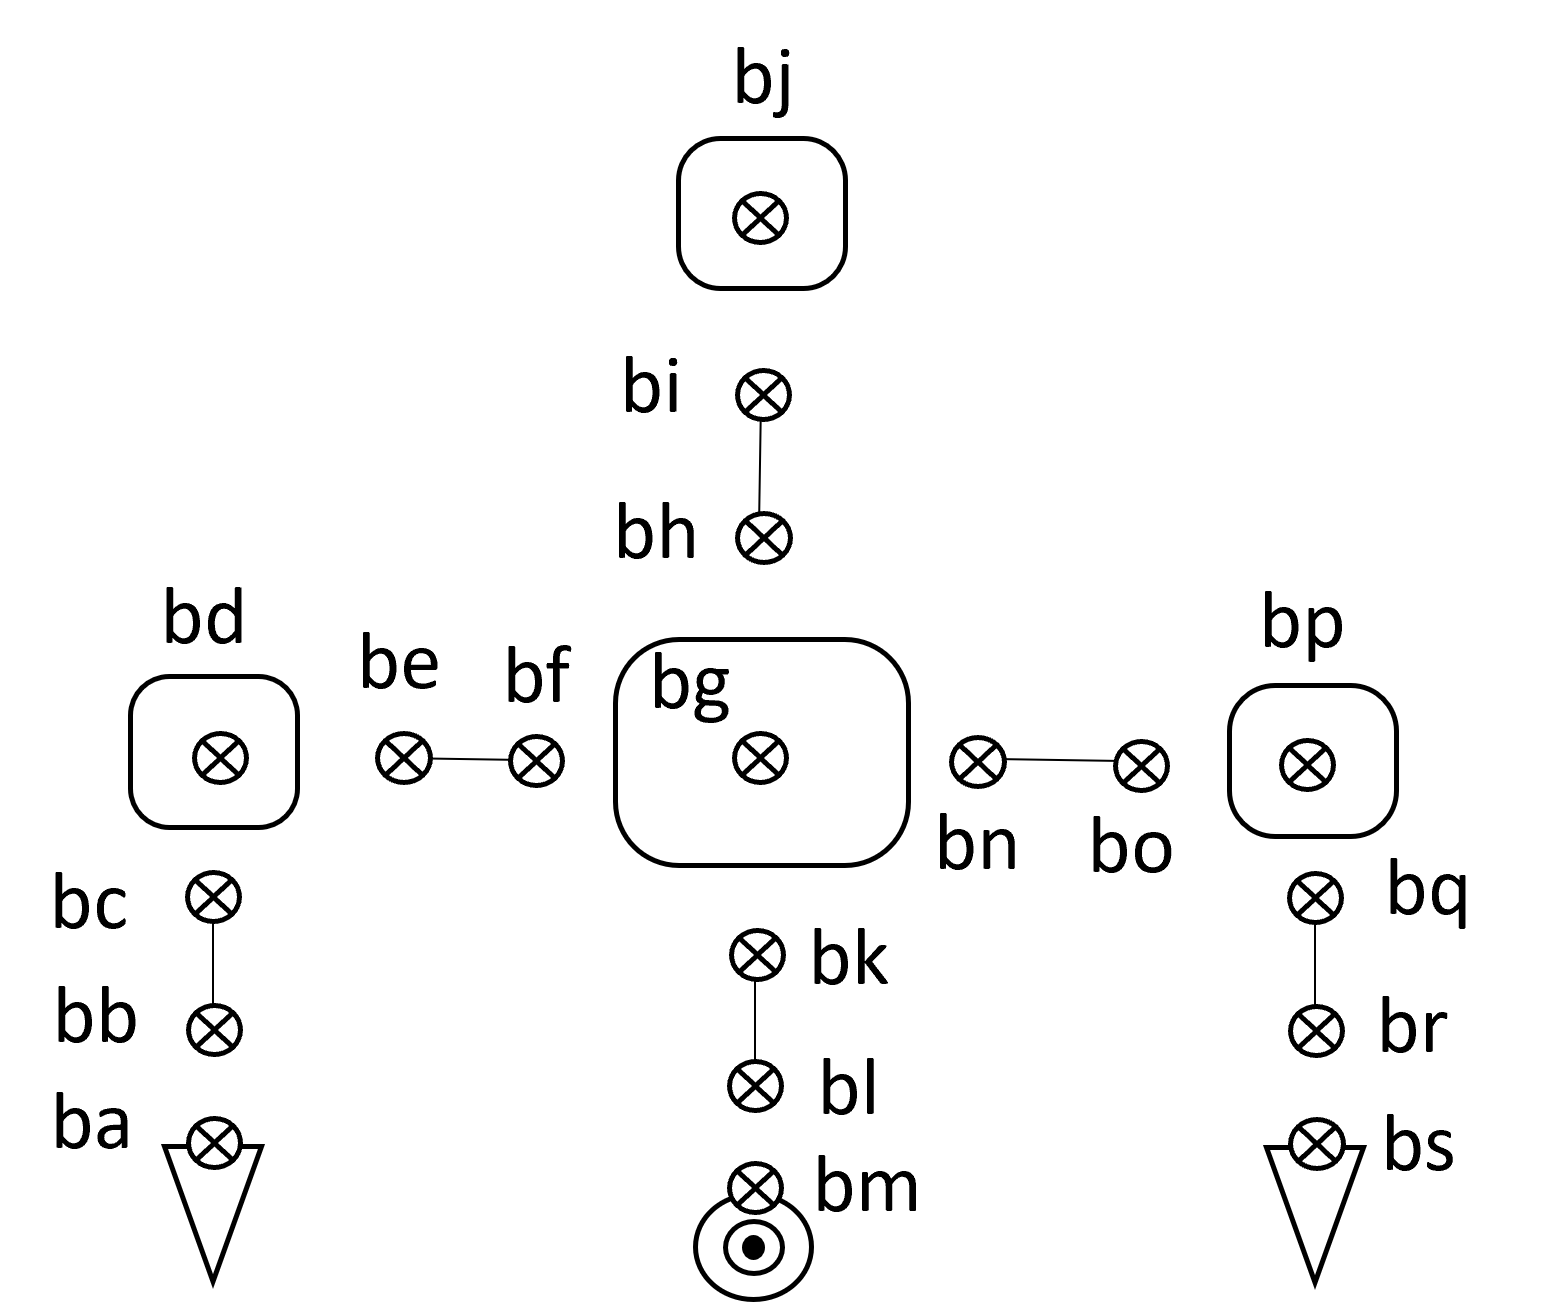
\includegraphics[width=0.35\textwidth]{Figures/host_boundaries.png}
    \caption{Definition of host boundaries. The boundary is represented by a circle crossed.}
    \label{fig:host_bound}
\end{figure}

\subsection{Boundaries mapping}

In the boundary mapping step, \ApproachName{} determine the relation between the boundaries of the organ and the host. From each boundary in the organ we map all possible connections that could have with boundaries of the host, including the possibility of not connecting the boundary to the host boundaries (Table.~\ref{tab:boundaries}). 

Table~\ref{tab:boundaries} map the compatible boundary connections between organ and host. The boundary b11 is a boundary from a \sq{Link} from the model and according to the metamodel it can connect to any \sq{Hull}, \sq{Weapon}, \sq{Weak Point} or remain unconnected. The boundaries b16 and b25 are both \sq{Hulls} and they can connect with any \sq{Link} or remain unconnected.

\begin{table}[h]
\centering
\resizebox{0.35\textwidth}{!}{
\begin{tabular}{|c|ll|}
\hline
{Organ boundary from donor} & \multicolumn{2}{c|}{{ \begin{tabular}[c]{@{}c@{}}Host \\      boundaries\end{tabular}}} \\ \hline
& \multicolumn{1}{c|}{ba} & \multicolumn{1}{c|}{bm} \\ \cline{2-3} 
& \multicolumn{1}{c|}{bd} & \multicolumn{1}{c|}{bp} \\ \cline{2-3} 
& \multicolumn{1}{c|}{bg} & \multicolumn{1}{c|}{bs} \\ \cline{2-3} 
\multirow{-4}{*}{b11} 
& \multicolumn{1}{c|}{bj} & \multicolumn{1}{c|}{Not connected} \\ \hline
& \multicolumn{1}{c|}{bb} & \multicolumn{1}{c|}{bc} \\ \cline{2-3} 
& \multicolumn{1}{c|}{be} & \multicolumn{1}{c|}{bf} \\ \cline{2-3} 
& \multicolumn{1}{c|}{bh} & \multicolumn{1}{c|}{bi} \\ \cline{2-3} 
& \multicolumn{1}{c|}{bk} & \multicolumn{1}{c|}{bl} \\ \cline{2-3} 
& \multicolumn{1}{c|}{bn} & \multicolumn{1}{c|}{bo} \\ \cline{2-3} 
\multirow{-6}{*}{\begin{tabular}[c]{@{}c@{}}b16\\    \\ b25\end{tabular}} 
& \multicolumn{2}{c|}{Not connected} \\ \hline
\end{tabular}}
\caption{Mapping  of compatible boundaries between organ and host.}
\label{tab:boundaries}
\end{table}

\subsection{Encoding}

We use a similar version of Blasco \etal that has been extended to work with transplantations. The size of the encoding in the previous work was 64 and in this work its size is of 150

\subsection{Genetic Operators}

Imhotep has three genetic operations (selection, crossover, and mutation) to generate new individuals. To select the individuals we use the ranking selection, which ranks the population by the objective function and takes the top 10\% of the individuals in the current population. The size of the population is limited to 100, i.e the selection will take 10 individuals to apply the operators.

We use a single, random, cut-point crossover. It starts by selecting and splitting two parent solutions at random. When two parent individuals are selected, a random cut point is determined to split them into two sub-vectors.
Then, the crossover creates two child solutions by putting the first part of the first parent with the second part of the second parent for the first child and putting the first part of the second parent with the second part of the first parent for the second child.

The new individual has a probability of 1/150 to mutate any value of the encoding. The probability is based on the size of the encoding of an individual which is 150 in our approach.

After all the operations have been applied, the new set of individuals are evaluated by the objective function and added to the population. The last individuals by ranking in the population are discarded to maintain the size of the population on 100. 

Figure.~\ref{fig:candidates} shows handmade new individuals that could results from our example.

\begin{figure}[h]
    \centering
    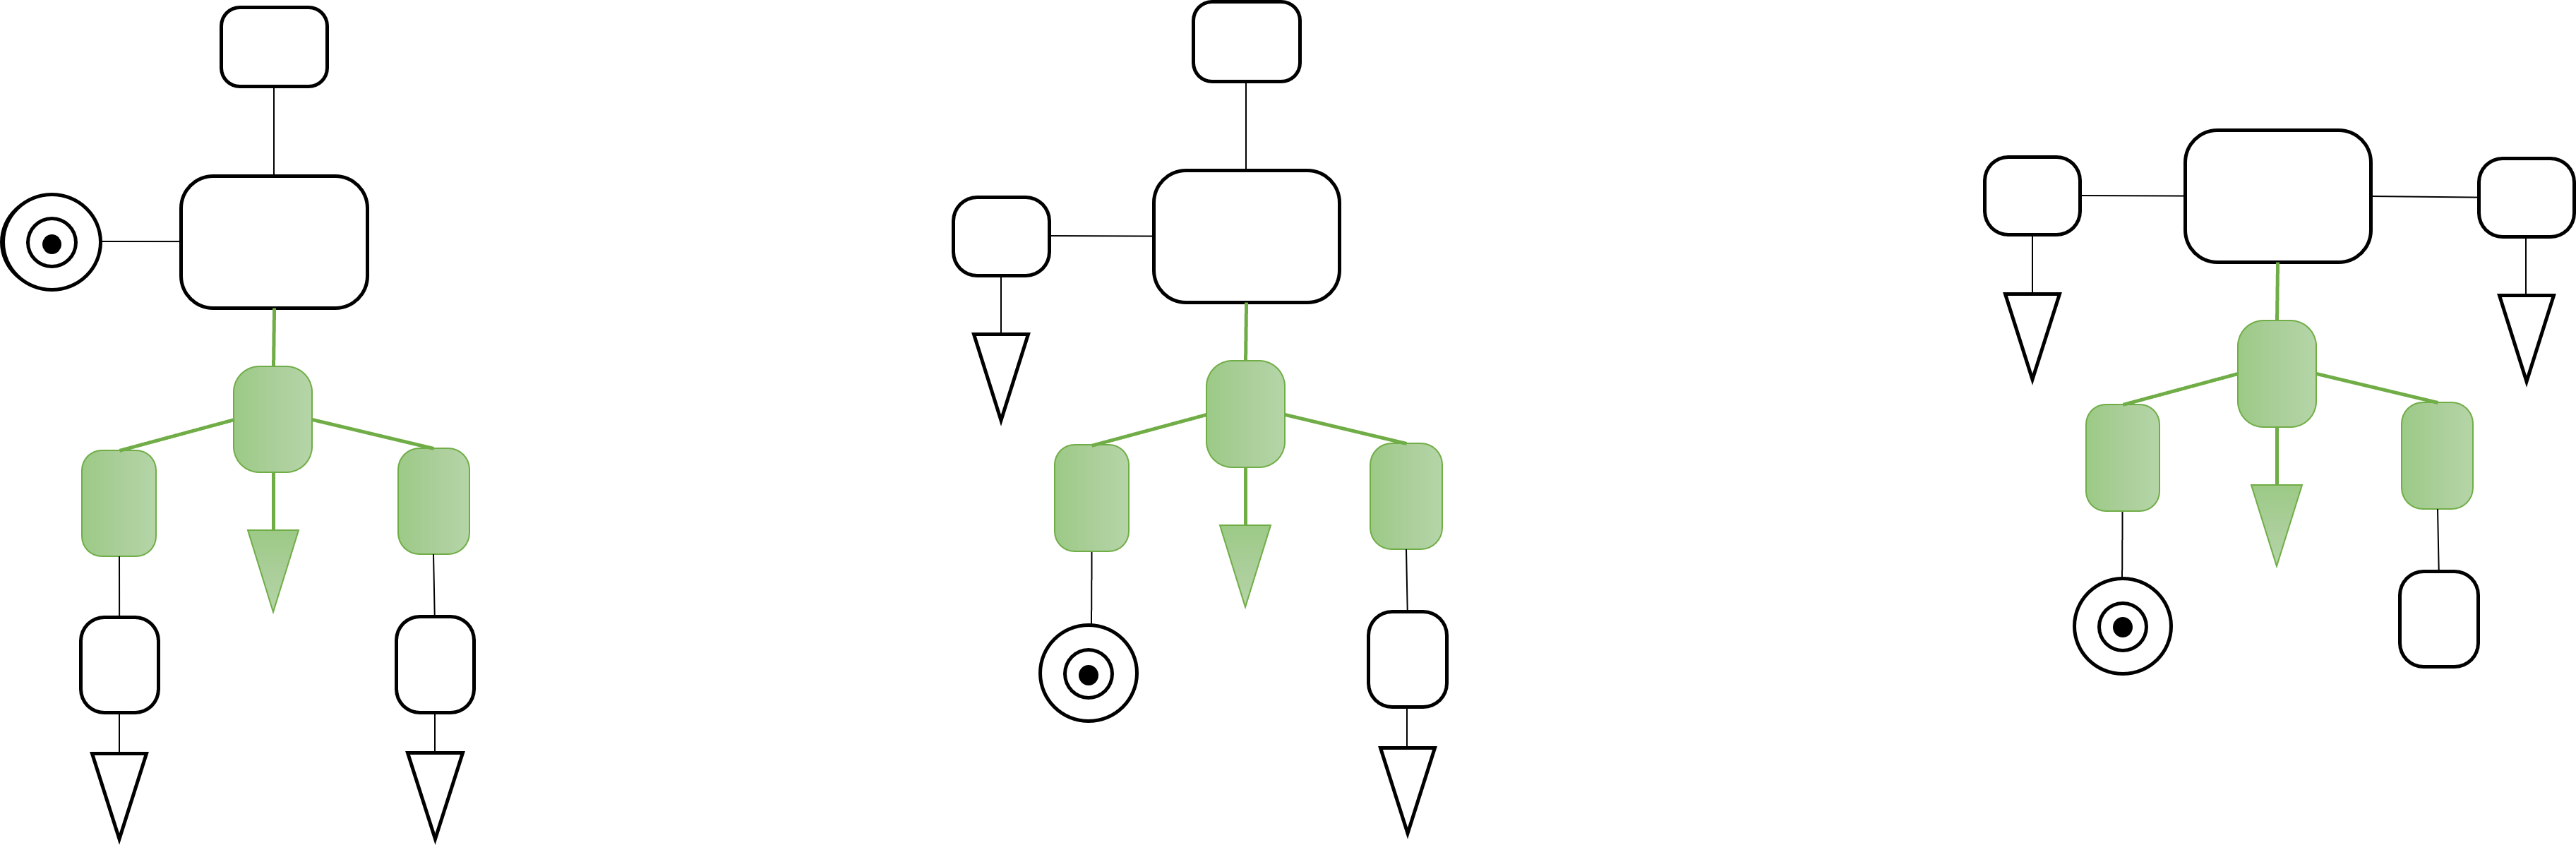
\includegraphics[width=0.45\textwidth]{Figures/candidates.png}
    \caption{Example of individuals to be evaluated by the objective function}
    \label{fig:candidates}
\end{figure}

\subsection{Objective function}

The objective function in \ApproachName{} assess the quality of each individual as a model. First, as done in previous work that use \CaseStudy{}~\cite{blasco2021evolutionary}, the models pass through a validation process followed by a quantitative measurement. In our work we assess quantitatively the objective function by two means; Test-based and Simulation-based objective functions. We use two different objective functions due to the differences in the the state-of-the-art of software transplantation and PCG. The state-of-the-art in software transplantation mainly work with Test-based objective function, while the state-of-the-art in NPCs PCG work with Simulation-based objective function.

The validation step before the Test-based or Simulation objective function is a requirement that \CaseStudy{} integrates in the game to avoid models with inconsistent data. The validity of the models is performed by a run-time interpreter that is part of the game. When the model is stated as non-valid the value of the objective function will be 0.0.

The models that passes the validation process will then be assess by Test-based and Simulation-based objective function.
For the Test-based objective function we ask the developers to provide the set of tests that they consider relevant to our work. The developers from \CaseStudy{} provided us a total of 243 test selected under they domain knowledge. The objective value will be retrieved when each individual pass through the 243 tests normalized in a scale of [0, 1] written this limitation. An individual which pass the 243 tests will obtain 1.0, and on the contrary if it does not pass any test will obtain 0.0.

On the other hand, the Simulation-based objective function as in Blasco \etal~\cite{blasco2021evolutionary} simulates an in game battle between the boss and a player. The information retrieved from the simulation is the data that the developers regard as relevant, using their domain knowledge. Hence, our approach takes into account the percentage of simulated player victories ($F_{Victory}$) and the percentage of simulated player health left once the player wins a duel ($F_{Health}$).
The calculation of $F_{Victory}$ and $F_{Health}$ is performed in the same
way as Blasco \etal~\cite{blasco2021evolutionary}:

$F_{Victory}$ is calculated as the difference between the number of human player victories ($V_{P}$) and the optimal number of victories (33\%, according to the developers of \CaseStudy{} and their criteria) ($V_{Optimal}$):
\begin{equation}
F_{Victory} = 1 -\frac{\mid V_{Optimal} - V_{P} \mid}{ V_{Optimal}}
\end{equation}

$F_{Health}$, which refers to completed duels that end in human player victories, is the average difference between the human player's health percentage once the duel is over ($\Theta_{P}$) and the optimal health level that the player should have at that point ($\Theta_{Optimal}$, 20\%, according to the developers):
\begin{equation}
F_{Health} = 1 - \frac{\sum\limits_{d=1}^{V_{P}}\frac{\mid \Theta_{Optimal} - \Theta_{P} \mid}{ \Theta_{Optimal}}}{V_{P}}
\end{equation}

$F_{Overall}$ is an average fitness value for a boss model that includes the fitness criteria described above. In the end, $F_{Overall}$ is a value in [0, 1] that is used to assess a boss model when our \ApproachName{} approach is applied to the \CaseStudy{} case study.

\begin{equation}
F_{Overall} = min( Validity, \frac{\sum\limits_{i=1}^{N}F_{i}}{N} )
\end{equation}
